%DO NOT MESS AROUND WITH THE CODE ON THIS PAGE UNLESS YOU %REALLY KNOW WHAT YOU ARE DOIN

\chapter{Implementation and Methodology} \label{Implementation and Methodology}

\section{Tools Used } \label{Tools Used }
\noindent The following Tools have been used for implementation.
\subsection{Microsoft Kinect v2 sensor} \label{Microsoft Kinect v2 sensor} 
\noindent Specifications of the Kinect are discussed in Chapter 3.
\subsection{Visual Studio 2015 Community Edition }\label{Visual Studio 2015 Community Edition }  
\noindent Microsoft Visual Studio is an integrated development environment (IDE) from Microsoft. It is used to develop computer programs for Microsoft Windows, as well as web sites, web apps, web services and mobile apps. Visual Studio uses Microsoft software development platforms such as Windows API, Windows Forms, Windows Presentation Foundation, Windows Store and Microsoft Silverlight. It can produce both native code and managed code.\\
\noindent Visual Studio supports different programming languages and allows the code editor and debugger to support (to varying degrees) nearly any programming language, provided a language-specific service exists. Built-in languages include C, C++and C++/CLI (via VisualC++), VB.NET (via VisualBasic.NET), C\# (via Visual C\#), and F\# (as of Visual Studio 2010). Support for other languages such as Python, Ruby, Node.js, and M among others is available via language services installed separately.
\noindent Microsoft provides the Kinect SDK and Kinect specific libraries to be used on Visual Studio. This is the reason we have chosen Visual Studio as our development platform as it makes interfacing the Kinect easy. 

\subsection{Vitruvius }\label{Vitruvius}
\noindent Vitruvius is an advanced kinect framework which provides a set of easy to use kinect utilities on Visual Studio and unity that simplify and speed up many aspects of Kinect for Windows App development.The product also alleviates alot of the heavy math associated with implementing motion tracking in advanced kinect apps.\\
Vitruvius lets you easily calculate joint angles and find the length of specified segments in 3D space, and the rotation of the body in the X, Y, Z axis.\\
Vitruvius also provides simplified bitmap manipulation and lets you take full advantage of the latest Kinect for Windows facial tracking and gesture detection for Windows human-computing interactions.\\ 
We used the Vitruvius Library on top of the SDK to simplify the maesuremnt of length and angles.

\subsection{Notepad++ }\label{Notepad++ } 
\noindent Notepad++ is a text editor and source code editor for use with Microsoft Windows. It supports tabbed editing, which allows working with multiple open files in a single window. Notepad++ is distributed as free software. It supports syntax highlighting and code folding for over 50 programming, scripting, and markup languages.\\
The skeletal data obtained from the SDK is stored in CSV format in a Notepad++.

\subsection{MATLAB R2015a }\label{MATLAB R2015a }
\noindent MATLAB is a multi-paradigm numerical computing environment and fourth-generation programming language. A proprietary programming language developed by MathWorks, MATLAB allows matrix manipulations, plotting of functions and data, implementation of algorithms, creation of user interfaces, and interfacing with programs written in other languages, including C, C++, C\#, Java, Fortran and Python.\\
MATLAB provides special toolboxes for applications such as Signal Processing and Communications, Control System Design and Analysis, Pattern Recognition, Classification Learner and other statistical modelling \\
The CSV format file is processed in MATLAB for gait feature extraction and classification. 

\section{Gait Features} \label{Gait Features } 
\noindent The Kinect SDK offers the detection and tracking of 25 different skeletal joints. The features that can be generated from these joints can broadly be classified as static and kinematic features.
The static features are the ones which do not change in time as a person is walking, for e.g. Height.
We define a set of 7 static features used in our study


\begin{table}
\centering
\begin{tabular}{| l | |p{5cm}|}
 \hline
SR No. & Static Features  \\ \hline
1 & Height \\ \hline
2 & Length of Full Arms \\ \hline
3 & Length of Fore Arms \\\hline
4 & Length of Upper Arms \\ \hline
5 & Length of Full Legs \\ \hline
6 & Length of Thighs \\\hline
7 & Length of Lower Legs \\ \hline

\end{tabular}
\caption{The set of static features}
\end{table}



\noindent Kinematic features basically involve distance and angle between joints while a person is walking. These value of these features constantly change during the walking and are shown to be periodic in nature.
We define a set of 8 kinematic features involving distance between joints 

\begin{table}
\centering
\begin{tabular}{| l | |p{6cm}|}
 \hline
SR No. & Features  \\ \hline
1 & Distance between ankles \\ \hline
2 & Distance between knees \\ \hline
3 & Distance between elbows \\\hline
4 & Distance between hands \\ \hline
5 & variance of head (along x) \\ \hline
6 & variance of head (along y) \\\hline
7 & variance of left knee (along y) \\ \hline
8 & variance of right knee (along y) \\ \hline
\end{tabular}
\caption{ kinematic features involving distance between joints}
\end{table}

\noindent When we talk about the features such as variance of head and knees along X and Y. We are trying to map the vertical and lateral oscillations of these skeleton joints.

\noindent Features involving angles are extracted during the walk but are not used in this study and will be discussed later. Here we would like to divide our implementations into two parts

\noindent$\bullet$ Part I  : This will deal with the experimental setup, design of the application using the Kinect SDK, logic behind measurements of static and kinematic features and their extraction.\\
The tasks discussed in Part I are implemented on Visual Studio

\noindent$\bullet$ Part II  : This involves the overhead processing on the gait features, classification and comparison on the performance of different classification algorithms.\\
These tasks are implemented on MATLAB


\section{Experimental Set up } \label{Experimental Set up }

\noindent 1) The Kinect was placed at height of 1.5m and the person was made to walk in front of the Kinect. The figure\ref{fig:exp.png} gives us a nice visual  representation of the setup.
\begin{figure}[h]
\centering
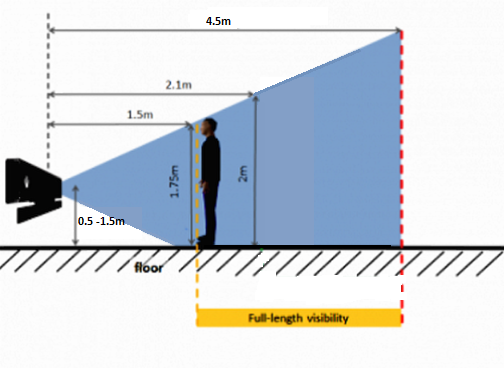
\includegraphics[scale=0.8]{exp.png}
\caption{Experimental Setup}
\label{fig:exp.png}
\end{figure}
\noindent 2) Initially, the person is made to stand in a straight posture at the maximum range of Kinect (close to 4.5m). Here the static feature readings are taken for a period of about 3 seconds.\\
3) Then the person is asked to walk straight towards the Kinect. We are interested in the kinematic features of the walk upto a distance of 1.5m from the Kinect, because within this range we are able to capture the motion of the entire body. Beyond this,some part of the joints always goes out of the frame.\\
4) Although the range of 3m (4.5-1.5 m) appears small. It is more than adequate to extract one complete gait cycle. The representation of this gait cycle is shown in Figure \ref{fig:exp.png}.\\

\section{Logic behind the measurement of static and kinematic features}\label{Logic behind the measurement of static and kinematic features} 
\subsection{Measurement of length between joints}\label{Measurement of length between joints} 

\noindent We refer back to the figure depicting all the body joints represented by the Kinect.
\begin{figure}[h]
\centering
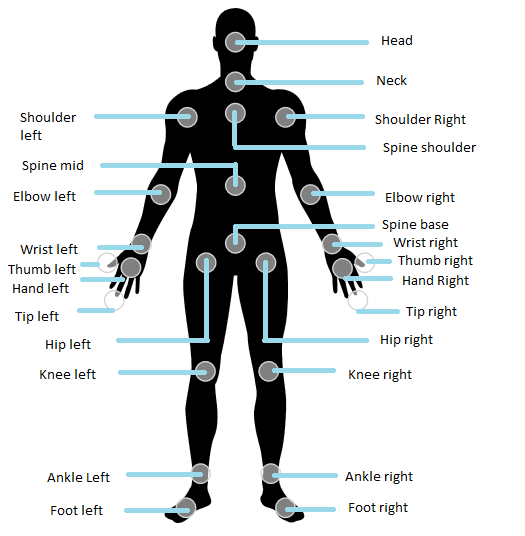
\includegraphics[scale=0.75]{Figbodjoints.png}
\caption{25 joints offered by Kinect}
\label{fig:Figbodjoints.png}
\end{figure}
\noindent For explanatory purposes we will show how height is measured. In principle same logic is applied to get other measurements and distances.\\
Kinect provides you with the coordinates (X, Y and Z) of 25 skeleton joints. We might think that a person's height is the distance from the head joint to a foot joint, right? This is fundamentally incorrect because users might stand with a bended knee, they might lean a bit to the left or to the right. If you try to calculate the distance defined from the head joint to one of the foot joints, you'll get a far from accurate result.\\
If we examine the skeleton joints as seen in figure \ref{fig:Figbodjoints.png} we'll notice that the height is the sum of the lengths of the following line segments:\\
\noindent$\bullet$   Head – Neck\\
$\bullet$	Neck – Spine Shoulder\\
$\bullet$	Spine Shoulder – Spine Mid\\
$\bullet$	Spine Mid – Spine Base\\
$\bullet$	Hip Left/Hip Right – Knee Left / Knee Right\\
$\bullet$	Knee Left / Knee Right – Ankle Left / Ankle Right\\
$\bullet$	Ankle Left / Ankle Right – Foot Left / Foot Right\\
Using (X,Y,Z) coordinates of each joint we can calculate the length of the line defined by two joints in the 3D space, simply by using the distance formula:

 D = $\sqrt{(x_{1}-x_{2})^2+ (y_{1}-y_{2})^2+(z_{1}-z_{2})^2}$

\noindent Pretty straightforward till here. But, how will we determine which leg corresponds to the most accurate user height? Hence we take the average of both the legs and then add this to the sum of the rest of the joints.\\
It should be noted that the height calculated in this case does not represent the true height because Kinect only gives you the centre of the head joint. It does not detect the end of the head for accurate measurements. Also height measured in this study excluded the foot left and right joints, as they being close to the floor gave readings prone to error.\\
Hence for all intent and purposes, whenever we talk about height in this study it will be the sum of the lengths of the line segments:

\noindent Head-$>$ Neck-$>$ Spine Shoulder-$>$ Spine Mid-$>$ Spine Base-$>$ HipLeft/HipRight-$>$ KneeLeft / KneeRight-$>$ AnkleLeft / AnkleRight\\ 
Where distances from the hip joint to the ankle joint gets averaged for the two legs.

\section{ Measurement of angles between joints} \label{ Measurement of angles between joints}
We present a new gait feature that provides us relative motion between two joints by computing the joint relative angles (JRA) over a complete gait cycle. JRA between two joints p1 and p2 can be defined as the angle formed by p1 and p2 with respect to a reference point r. Given the coordinates of 3 points p1, p2, and r in a 3-D space the angle p1, p2 formed by p1 --$>$ r --$>$ p2 can be calculated as

\begin{figure}[h]
\centering
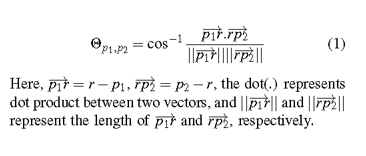
\includegraphics[scale=0.9]{equation.png}

\end{figure}
\noindent The SPINE\_ BASE joint was selected as the reference point, since it remains almost stationary during walking.\\                                           For the 25 skeletal joints, there is a total of 300 possible joint-pair combinations, which is a high-dimensional feature space. In our study we left out JRA involving 5 joints:  Hand Left/Right, Tip Left/Right and SpineBase. The position of the 4 former joints are usually irrelevant to gait and the latter if included would have given us just 2 joints(a line) instead of 3,which is required for an angle. So we are left with 20 joints, which gives us a total of 190 possible combinations.\\
In addition, out of these 190 not all joint-pair is relevant in gait feature representation. For example, JRAs between the SpineShoulder and the SpineMid joints does not represent any information related to human gait, since both these joints remain almost stationary when a person walks. Therefore, identifying the skeletal joint pairs that are relevant to human gait motion is imperative. The following figure gives an example of a JRA. \\
\begin{figure}[h]
\centering
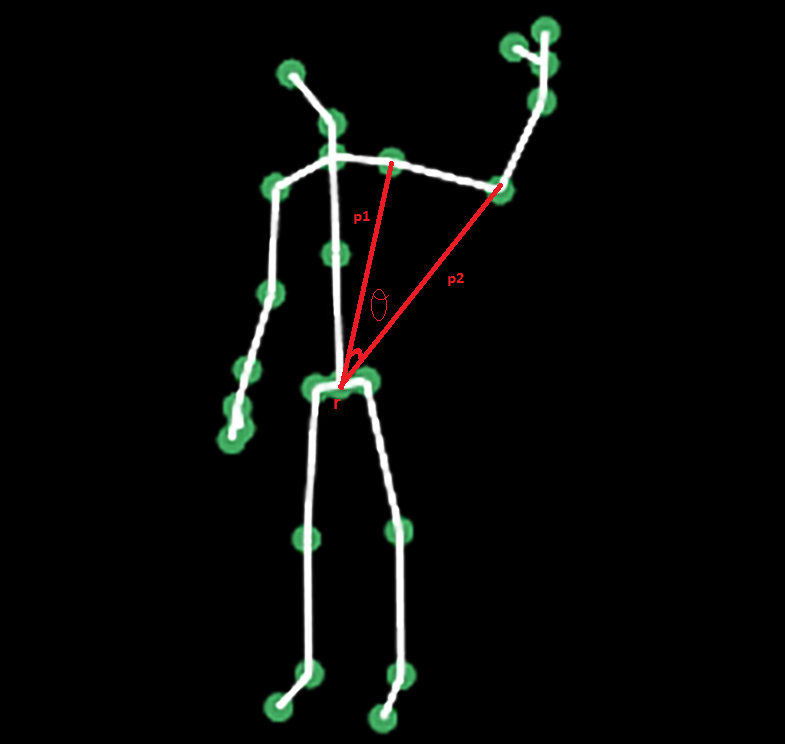
\includegraphics[scale=0.5]{angle.png}
\caption{JRA between Shoulder Left and Elbow Left}
\end{figure}


\section{Design of the App } \label{ Design of the App} 
\noindent We designed a windows application on Visual Studio using the Kinect SDK for the purpose of extracting skeletal data and gait features which were discussed in the preceding sections. We named our App “TRACE”.

Here is the front page of TRACE. It has only one circular button. When pressed leads to the next page where the actual extraction happens.

\begin{figure}[h]
\centering
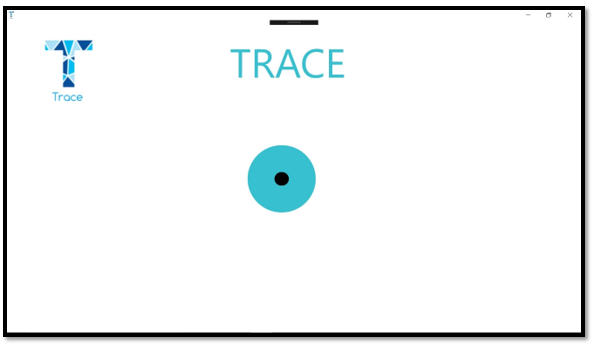
\includegraphics[scale=0.7]{trace.png}
\caption{Trace}
\end{figure} 

\begin{figure}[h]
\centering
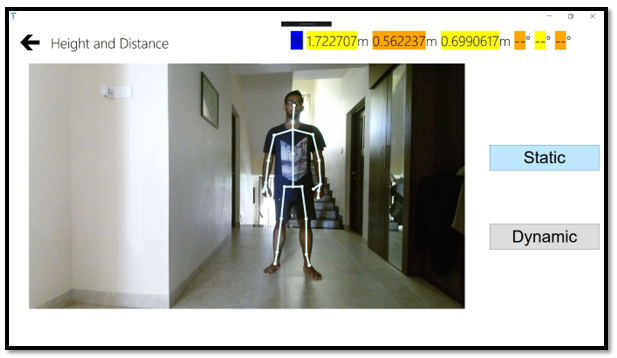
\includegraphics[scale=0.7]{john.png}
\caption{Skeletal View}
\end{figure}

This Page has two buttons on the right for capturing the static and kinematic/dynamic data respectively. \\
Data displayed on the top right is basically for the operator to know that the process is working fine. The number in blue indicates the joints currently being tracked by the Kinect. The next 3 are distance measurement between various joints. The final 3 are used for displaying angles, currently null since only the static button has been pressed.\\
The two figures below show how TRACE writes the static and dynamic data in CSV format. Each new line represents each frame of the walking sequence captured.\\
\begin{figure}[h]
\centering
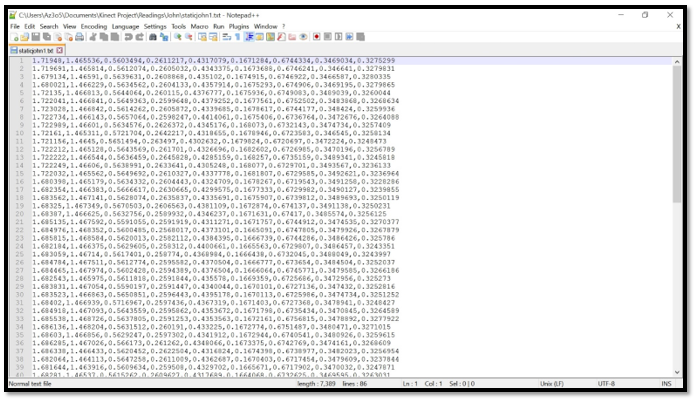
\includegraphics[scale=0.7]{static.png}
\caption{Static data in CSV format}
\end{figure}

\begin{figure}[h]
\centering
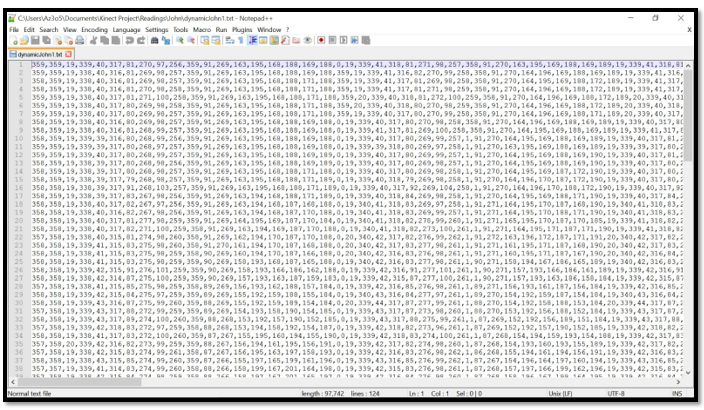
\includegraphics[scale=0.7]{dynamic.png}
\caption{Dynamic data in CSV format}
\end{figure}










